% Options for packages loaded elsewhere
\PassOptionsToPackage{unicode}{hyperref}
\PassOptionsToPackage{hyphens}{url}
%
\documentclass[
]{article}
\author{}
\date{\vspace{-2.5em}}

\usepackage{amsmath,amssymb}
\usepackage{lmodern}
\usepackage{iftex}
\ifPDFTeX
  \usepackage[T1]{fontenc}
  \usepackage[utf8]{inputenc}
  \usepackage{textcomp} % provide euro and other symbols
\else % if luatex or xetex
  \usepackage{unicode-math}
  \defaultfontfeatures{Scale=MatchLowercase}
  \defaultfontfeatures[\rmfamily]{Ligatures=TeX,Scale=1}
\fi
% Use upquote if available, for straight quotes in verbatim environments
\IfFileExists{upquote.sty}{\usepackage{upquote}}{}
\IfFileExists{microtype.sty}{% use microtype if available
  \usepackage[]{microtype}
  \UseMicrotypeSet[protrusion]{basicmath} % disable protrusion for tt fonts
}{}
\makeatletter
\@ifundefined{KOMAClassName}{% if non-KOMA class
  \IfFileExists{parskip.sty}{%
    \usepackage{parskip}
  }{% else
    \setlength{\parindent}{0pt}
    \setlength{\parskip}{6pt plus 2pt minus 1pt}}
}{% if KOMA class
  \KOMAoptions{parskip=half}}
\makeatother
\usepackage{xcolor}
\IfFileExists{xurl.sty}{\usepackage{xurl}}{} % add URL line breaks if available
\IfFileExists{bookmark.sty}{\usepackage{bookmark}}{\usepackage{hyperref}}
\hypersetup{
  hidelinks,
  pdfcreator={LaTeX via pandoc}}
\urlstyle{same} % disable monospaced font for URLs
\usepackage[margin=1in]{geometry}
\usepackage{color}
\usepackage{fancyvrb}
\newcommand{\VerbBar}{|}
\newcommand{\VERB}{\Verb[commandchars=\\\{\}]}
\DefineVerbatimEnvironment{Highlighting}{Verbatim}{commandchars=\\\{\}}
% Add ',fontsize=\small' for more characters per line
\usepackage{framed}
\definecolor{shadecolor}{RGB}{248,248,248}
\newenvironment{Shaded}{\begin{snugshade}}{\end{snugshade}}
\newcommand{\AlertTok}[1]{\textcolor[rgb]{0.94,0.16,0.16}{#1}}
\newcommand{\AnnotationTok}[1]{\textcolor[rgb]{0.56,0.35,0.01}{\textbf{\textit{#1}}}}
\newcommand{\AttributeTok}[1]{\textcolor[rgb]{0.77,0.63,0.00}{#1}}
\newcommand{\BaseNTok}[1]{\textcolor[rgb]{0.00,0.00,0.81}{#1}}
\newcommand{\BuiltInTok}[1]{#1}
\newcommand{\CharTok}[1]{\textcolor[rgb]{0.31,0.60,0.02}{#1}}
\newcommand{\CommentTok}[1]{\textcolor[rgb]{0.56,0.35,0.01}{\textit{#1}}}
\newcommand{\CommentVarTok}[1]{\textcolor[rgb]{0.56,0.35,0.01}{\textbf{\textit{#1}}}}
\newcommand{\ConstantTok}[1]{\textcolor[rgb]{0.00,0.00,0.00}{#1}}
\newcommand{\ControlFlowTok}[1]{\textcolor[rgb]{0.13,0.29,0.53}{\textbf{#1}}}
\newcommand{\DataTypeTok}[1]{\textcolor[rgb]{0.13,0.29,0.53}{#1}}
\newcommand{\DecValTok}[1]{\textcolor[rgb]{0.00,0.00,0.81}{#1}}
\newcommand{\DocumentationTok}[1]{\textcolor[rgb]{0.56,0.35,0.01}{\textbf{\textit{#1}}}}
\newcommand{\ErrorTok}[1]{\textcolor[rgb]{0.64,0.00,0.00}{\textbf{#1}}}
\newcommand{\ExtensionTok}[1]{#1}
\newcommand{\FloatTok}[1]{\textcolor[rgb]{0.00,0.00,0.81}{#1}}
\newcommand{\FunctionTok}[1]{\textcolor[rgb]{0.00,0.00,0.00}{#1}}
\newcommand{\ImportTok}[1]{#1}
\newcommand{\InformationTok}[1]{\textcolor[rgb]{0.56,0.35,0.01}{\textbf{\textit{#1}}}}
\newcommand{\KeywordTok}[1]{\textcolor[rgb]{0.13,0.29,0.53}{\textbf{#1}}}
\newcommand{\NormalTok}[1]{#1}
\newcommand{\OperatorTok}[1]{\textcolor[rgb]{0.81,0.36,0.00}{\textbf{#1}}}
\newcommand{\OtherTok}[1]{\textcolor[rgb]{0.56,0.35,0.01}{#1}}
\newcommand{\PreprocessorTok}[1]{\textcolor[rgb]{0.56,0.35,0.01}{\textit{#1}}}
\newcommand{\RegionMarkerTok}[1]{#1}
\newcommand{\SpecialCharTok}[1]{\textcolor[rgb]{0.00,0.00,0.00}{#1}}
\newcommand{\SpecialStringTok}[1]{\textcolor[rgb]{0.31,0.60,0.02}{#1}}
\newcommand{\StringTok}[1]{\textcolor[rgb]{0.31,0.60,0.02}{#1}}
\newcommand{\VariableTok}[1]{\textcolor[rgb]{0.00,0.00,0.00}{#1}}
\newcommand{\VerbatimStringTok}[1]{\textcolor[rgb]{0.31,0.60,0.02}{#1}}
\newcommand{\WarningTok}[1]{\textcolor[rgb]{0.56,0.35,0.01}{\textbf{\textit{#1}}}}
\usepackage{longtable,booktabs,array}
\usepackage{calc} % for calculating minipage widths
% Correct order of tables after \paragraph or \subparagraph
\usepackage{etoolbox}
\makeatletter
\patchcmd\longtable{\par}{\if@noskipsec\mbox{}\fi\par}{}{}
\makeatother
% Allow footnotes in longtable head/foot
\IfFileExists{footnotehyper.sty}{\usepackage{footnotehyper}}{\usepackage{footnote}}
\makesavenoteenv{longtable}
\usepackage{graphicx}
\makeatletter
\def\maxwidth{\ifdim\Gin@nat@width>\linewidth\linewidth\else\Gin@nat@width\fi}
\def\maxheight{\ifdim\Gin@nat@height>\textheight\textheight\else\Gin@nat@height\fi}
\makeatother
% Scale images if necessary, so that they will not overflow the page
% margins by default, and it is still possible to overwrite the defaults
% using explicit options in \includegraphics[width, height, ...]{}
\setkeys{Gin}{width=\maxwidth,height=\maxheight,keepaspectratio}
% Set default figure placement to htbp
\makeatletter
\def\fps@figure{htbp}
\makeatother
\setlength{\emergencystretch}{3em} % prevent overfull lines
\providecommand{\tightlist}{%
  \setlength{\itemsep}{0pt}\setlength{\parskip}{0pt}}
\setcounter{secnumdepth}{5}
\ifLuaTeX
  \usepackage{selnolig}  % disable illegal ligatures
\fi

\begin{document}

\hypertarget{appendix-c-model-diagnosis}{%
\subsection*{Appendix C: Model diagnosis}\label{appendix-c-model-diagnosis}}
\addcontentsline{toc}{subsection}{Appendix C: Model diagnosis}

\hypertarget{population-aboveground-mass-and-stand-density}{%
\subsubsection*{Population aboveground mass and stand density}\label{population-aboveground-mass-and-stand-density}}
\addcontentsline{toc}{subsubsection}{Population aboveground mass and stand density}

\begin{Shaded}
\begin{Highlighting}[]
\DocumentationTok{\#\#\#\# Did crop identity and corn weed management affect AMATA aboveground mass in 2018? \#\#\#\#}

\NormalTok{pop\_biom18 }\OtherTok{\textless{}{-}} \FunctionTok{lm}\NormalTok{(}\FunctionTok{log}\NormalTok{(g\_m\_sq }\SpecialCharTok{+} \FloatTok{0.00025}\NormalTok{) }\SpecialCharTok{\textasciitilde{}}\NormalTok{ Block }\SpecialCharTok{+}\NormalTok{ Crop\_ID}\SpecialCharTok{*}\NormalTok{Corn\_weed\_management, }
                   \AttributeTok{data =}\NormalTok{ amata18)}
\FunctionTok{resid\_panel}\NormalTok{(pop\_biom18) }
\end{Highlighting}
\end{Shaded}

\begin{figure}
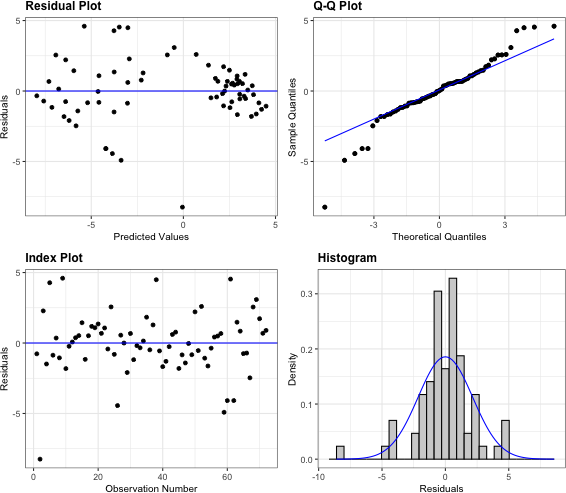
\includegraphics[width=1\linewidth]{AppendixC_model_diagnosis_files/figure-latex/pop-biom-18-1} \caption{Diagnosis plot for a model of the effects of crop identity and corn weed management on 2018 population aboveground mass.}\label{fig:pop-biom-18}
\end{figure}

\begin{Shaded}
\begin{Highlighting}[]
\DocumentationTok{\#\#\#\# Did crop identity and corn weed management affect AMATA aboveground mass in 2018? \#\#\#\#}

\NormalTok{pop\_biom19}\OtherTok{\textless{}{-}} \FunctionTok{lm}\NormalTok{(}\FunctionTok{log}\NormalTok{(g\_m\_sq }\SpecialCharTok{+} \FloatTok{0.002}\NormalTok{) }\SpecialCharTok{\textasciitilde{}}\NormalTok{ Block }\SpecialCharTok{+}\NormalTok{ Crop\_ID}\SpecialCharTok{*}\NormalTok{Corn\_weed\_management,}
                   \AttributeTok{data =}\NormalTok{ amata19)}

\FunctionTok{resid\_panel}\NormalTok{(pop\_biom19) }
\end{Highlighting}
\end{Shaded}

\begin{figure}
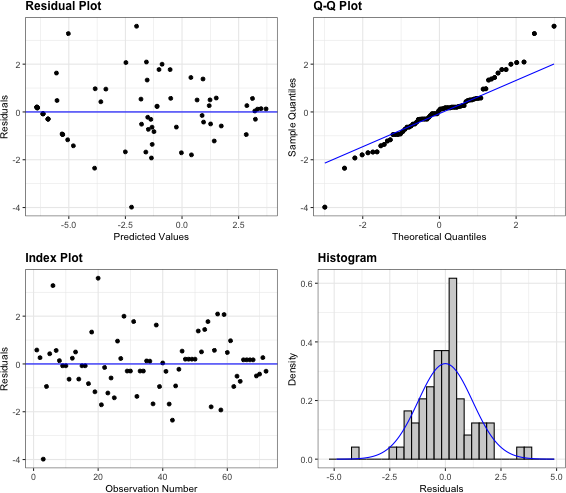
\includegraphics[width=1\linewidth]{AppendixC_model_diagnosis_files/figure-latex/pop-biom-19-1} \caption{Diagnosis plot for a model of the effects of crop identity and corn weed management on 2019 population aboveground mass.}\label{fig:pop-biom-19}
\end{figure}

\begin{Shaded}
\begin{Highlighting}[]
\DocumentationTok{\#\#\#\# Did crop identity and corn weed management affect AMATA density in 2018? \#\#\#\#}

\NormalTok{pop\_dens18 }\OtherTok{\textless{}{-}} \FunctionTok{lm}\NormalTok{(}\FunctionTok{log}\NormalTok{(plant\_m\_sq }\SpecialCharTok{+} \FloatTok{0.025}\NormalTok{) }\SpecialCharTok{\textasciitilde{}}\NormalTok{ Block }\SpecialCharTok{+}\NormalTok{ Crop\_ID}\SpecialCharTok{*}\NormalTok{Corn\_weed\_management, }
                   \AttributeTok{data =}\NormalTok{ amata18)}

\FunctionTok{resid\_panel}\NormalTok{(pop\_dens18) }
\end{Highlighting}
\end{Shaded}

\begin{figure}
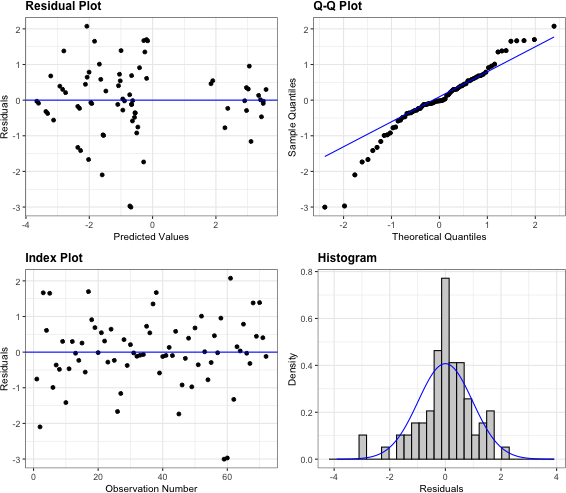
\includegraphics[width=1\linewidth]{AppendixC_model_diagnosis_files/figure-latex/pop-dens-18-1} \caption{Diagnosis plot for a model of the effects of crop identity and corn weed management on 2018 population density.}\label{fig:pop-dens-18}
\end{figure}

\begin{Shaded}
\begin{Highlighting}[]
\DocumentationTok{\#\#\#\# Did crop identity and corn weed management affect AMATA density in 2019? \#\#\#\#}
\NormalTok{pop\_dens19 }\OtherTok{\textless{}{-}} \FunctionTok{lm}\NormalTok{(}\FunctionTok{log}\NormalTok{(plant\_m\_sq }\SpecialCharTok{+} \FloatTok{0.025}\NormalTok{) }\SpecialCharTok{\textasciitilde{}}\NormalTok{ Block }\SpecialCharTok{+}\NormalTok{ Crop\_ID}\SpecialCharTok{*}\NormalTok{Corn\_weed\_management,}
                   \AttributeTok{data =}\NormalTok{ amata19)}

\FunctionTok{resid\_panel}\NormalTok{(pop\_dens19) }
\end{Highlighting}
\end{Shaded}

\begin{figure}
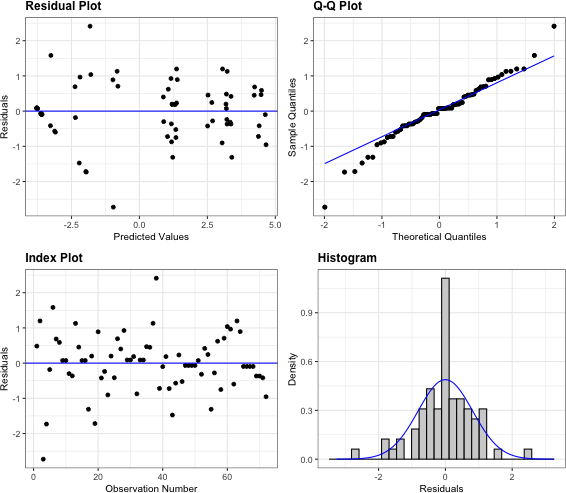
\includegraphics[width=1\linewidth]{AppendixC_model_diagnosis_files/figure-latex/pop-dens-19-1} \caption{Diagnosis plot for a model of the effects of crop identity and corn weed management on 2019 population density.}\label{fig:pop-dens-19}
\end{figure}

\hypertarget{population-sex-ratio}{%
\subsubsection*{Population sex ratio}\label{population-sex-ratio}}
\addcontentsline{toc}{subsubsection}{Population sex ratio}

\begin{Shaded}
\begin{Highlighting}[]
\DocumentationTok{\#\#\#\# Did crop identity and corn weed management had any effect on 2018 population sex ratio? \#\#\#\#}
\NormalTok{sexed18.glm }\OtherTok{\textless{}{-}} \FunctionTok{glm}\NormalTok{(}\FunctionTok{cbind}\NormalTok{(Female, Male) }\SpecialCharTok{\textasciitilde{}}\NormalTok{ Block }\SpecialCharTok{+}\NormalTok{ Crop\_ID}\SpecialCharTok{*}\NormalTok{Corn\_weed\_management,}
  \AttributeTok{data=}\NormalTok{amata18, }\AttributeTok{family=}\FunctionTok{quasibinomial}\NormalTok{(}\AttributeTok{link =} \StringTok{"logit"}\NormalTok{))}

\FunctionTok{glm.diag.plots}\NormalTok{(sexed18.glm) }\CommentTok{\#in boot package}
\end{Highlighting}
\end{Shaded}

\begin{figure}
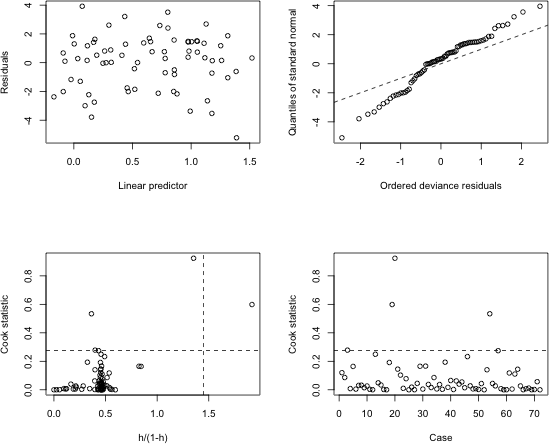
\includegraphics[width=1\linewidth]{AppendixC_model_diagnosis_files/figure-latex/sexr18-1} \caption{Diagnosis plot for a model of the effects of crop identity, corn weed management, and population aboveground mass on 2018 population sex ratio. Deviance = 165.91.}\label{fig:sexr18}
\end{figure}

\begin{Shaded}
\begin{Highlighting}[]
\CommentTok{\# deviance(sexed18.glm) \# 165.9}
\end{Highlighting}
\end{Shaded}

\begin{Shaded}
\begin{Highlighting}[]
\DocumentationTok{\#\#\#\# Did population aboveground mass, crop identity and corn weed management had any effect on 2018 population sex ratio? \#\#\#\#}

\NormalTok{sexr18\_biom\_glm }\OtherTok{\textless{}{-}} \FunctionTok{glm}\NormalTok{(}\FunctionTok{cbind}\NormalTok{(Female, Male) }\SpecialCharTok{\textasciitilde{}}\NormalTok{ Block }\SpecialCharTok{+}\NormalTok{  Crop\_ID }\SpecialCharTok{+}\NormalTok{ Corn\_weed\_management }\SpecialCharTok{+} 
                          \FunctionTok{log}\NormalTok{(g\_m\_sq }\SpecialCharTok{+} \FloatTok{0.00025}\NormalTok{) }\SpecialCharTok{+}
\NormalTok{                        Crop\_ID}\SpecialCharTok{:}\NormalTok{Corn\_weed\_management }\SpecialCharTok{+} 
                        \FunctionTok{log}\NormalTok{(g\_m\_sq }\SpecialCharTok{+} \FloatTok{0.00025}\NormalTok{)}\SpecialCharTok{:}\NormalTok{Crop\_ID }\SpecialCharTok{+}
                        \FunctionTok{log}\NormalTok{(g\_m\_sq }\SpecialCharTok{+} \FloatTok{0.00025}\NormalTok{)}\SpecialCharTok{:}\NormalTok{Corn\_weed\_management }\SpecialCharTok{+}
                        \FunctionTok{log}\NormalTok{(g\_m\_sq }\SpecialCharTok{+} \FloatTok{0.00025}\NormalTok{)}\SpecialCharTok{:}\NormalTok{Crop\_ID}\SpecialCharTok{:}\NormalTok{Corn\_weed\_management ,}
  \AttributeTok{data=}\NormalTok{amata18, }\AttributeTok{family=}\FunctionTok{quasibinomial}\NormalTok{(}\AttributeTok{link =} \StringTok{"logit"}\NormalTok{))}

\FunctionTok{glm.diag.plots}\NormalTok{(sexr18\_biom\_glm)}
\end{Highlighting}
\end{Shaded}

\begin{figure}
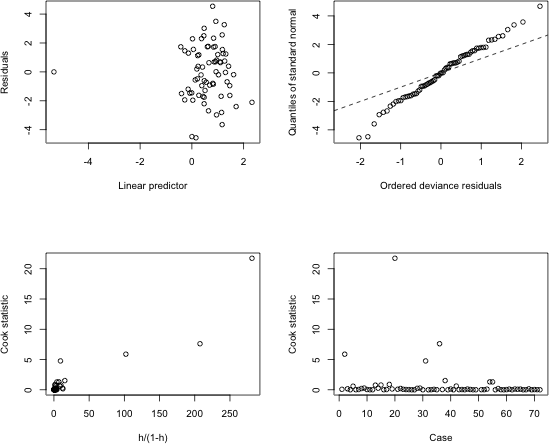
\includegraphics[width=1\linewidth]{AppendixC_model_diagnosis_files/figure-latex/sexr18-biom-1} \caption{Diagnosis plot for a model of the effects of crop identity, corn weed management, and population aboveground mass on 2018 population sex ratio. Deviance = 104.26.}\label{fig:sexr18-biom}
\end{figure}

\begin{Shaded}
\begin{Highlighting}[]
\CommentTok{\#deviance(sexr18\_biom\_glm3) \# 104.256}
\end{Highlighting}
\end{Shaded}

\begin{Shaded}
\begin{Highlighting}[]
\DocumentationTok{\#\#\#\# Did crop identity, corn weed management and plant density affect AMATA aboveground mass in 2018? \#\#\#\#}

\NormalTok{sexr18\_dens\_glm3 }\OtherTok{\textless{}{-}} \FunctionTok{glm}\NormalTok{(}\FunctionTok{cbind}\NormalTok{(Female, Male) }\SpecialCharTok{\textasciitilde{}}\NormalTok{ Block  }\SpecialCharTok{+}\NormalTok{ Crop\_ID }\SpecialCharTok{+}\NormalTok{ Corn\_weed\_management }\SpecialCharTok{+}
                          \SpecialCharTok{+} \FunctionTok{log}\NormalTok{(plant\_m\_sq }\SpecialCharTok{+} \FloatTok{0.025}\NormalTok{)  }\SpecialCharTok{+}
\NormalTok{                        Crop\_ID}\SpecialCharTok{:}\NormalTok{Corn\_weed\_management }\SpecialCharTok{+} 
                        \FunctionTok{log}\NormalTok{(plant\_m\_sq }\SpecialCharTok{+} \FloatTok{0.025}\NormalTok{)}\SpecialCharTok{:}\NormalTok{Crop\_ID }\SpecialCharTok{+}
                        \FunctionTok{log}\NormalTok{(plant\_m\_sq }\SpecialCharTok{+} \FloatTok{0.025}\NormalTok{)}\SpecialCharTok{:}\NormalTok{Corn\_weed\_management }\SpecialCharTok{+}
                        \FunctionTok{log}\NormalTok{(plant\_m\_sq }\SpecialCharTok{+} \FloatTok{0.025}\NormalTok{)}\SpecialCharTok{:}\NormalTok{Crop\_ID}\SpecialCharTok{:}\NormalTok{Corn\_weed\_management ,}
  \AttributeTok{data=}\NormalTok{amata18, }\AttributeTok{family=}\FunctionTok{quasibinomial}\NormalTok{(}\AttributeTok{link =} \StringTok{"logit"}\NormalTok{))}

\FunctionTok{glm.diag.plots}\NormalTok{(sexr18\_dens\_glm3)}
\end{Highlighting}
\end{Shaded}

\begin{figure}
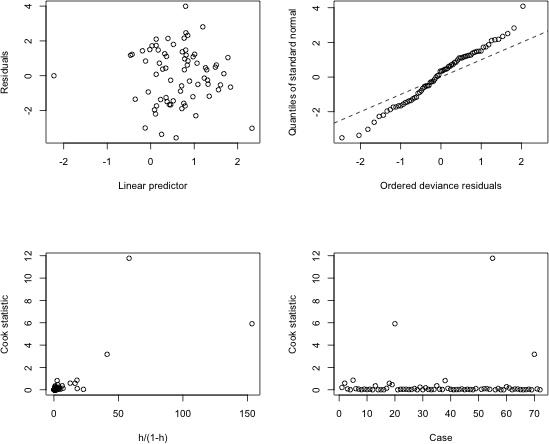
\includegraphics[width=1\linewidth]{AppendixC_model_diagnosis_files/figure-latex/sexr18-dens-1} \caption{Diagnosis plot for a model of the effects of crop identity, corn weed management, and population density on 2018 population sex ratio. Deviance = 82.12.}\label{fig:sexr18-dens}
\end{figure}

\begin{Shaded}
\begin{Highlighting}[]
\CommentTok{\# GLM link function explained \textless{}http://web.pdx.edu/\textasciitilde{}newsomj/cdaclass/ho\_glm.pdf\textgreater{}}

\CommentTok{\# deviance(sexr18\_dens\_glm3 )  \# = 82.12}
\end{Highlighting}
\end{Shaded}

\hypertarget{individual-female-aboveground-mass-and-fecundity}{%
\subsubsection*{Individual female aboveground mass and fecundity}\label{individual-female-aboveground-mass-and-fecundity}}
\addcontentsline{toc}{subsubsection}{Individual female aboveground mass and fecundity}

\begin{Shaded}
\begin{Highlighting}[]
\DocumentationTok{\#\#\#\# Did crop identity and corn weed management affect individual aboveground mass? \#\#\#\#}
\CommentTok{\# Keep rows with no NAs only, fecundity18\_b for Biomass}

\NormalTok{fecundity18\_b }\OtherTok{\textless{}{-}}\NormalTok{ fecundity18[}\FunctionTok{complete.cases}\NormalTok{(fecundity18}\SpecialCharTok{$}\NormalTok{Biomass), ]}
\CommentTok{\# min(fecundity18\_b$Biomass[fecundity18\_b$Biomass \textgreater{} 0])}

\NormalTok{biomass.gls }\OtherTok{\textless{}{-}} \FunctionTok{gls}\NormalTok{(}\FunctionTok{log}\NormalTok{(Biomass }\SpecialCharTok{+} \FloatTok{0.005}\NormalTok{) }\SpecialCharTok{\textasciitilde{}}\NormalTok{ Block }\SpecialCharTok{+}\NormalTok{ Crop\_ID }\SpecialCharTok{+} 
\NormalTok{                     Corn\_weed\_management }\SpecialCharTok{+}\NormalTok{ Crop\_ID}\SpecialCharTok{:}\NormalTok{Corn\_weed\_management,}
                   \AttributeTok{correlation=}\FunctionTok{corCompSymm}\NormalTok{(}\AttributeTok{form=} \SpecialCharTok{\textasciitilde{}}\DecValTok{1} \SpecialCharTok{|}\NormalTok{ bt), }\CommentTok{\#identifies each treatment within block}
  \AttributeTok{data=}\NormalTok{fecundity18\_b)}

\CommentTok{\# Ho testing reference \textless{}http://web.pdx.edu/\textasciitilde{}newsomj/cdaclass/ho\_glm.pdf\textgreater{}}

\FunctionTok{diag\_biom}\NormalTok{(biomass.gls, }\AttributeTok{tag=} \StringTok{""}\NormalTok{)}
\end{Highlighting}
\end{Shaded}

\begin{figure}
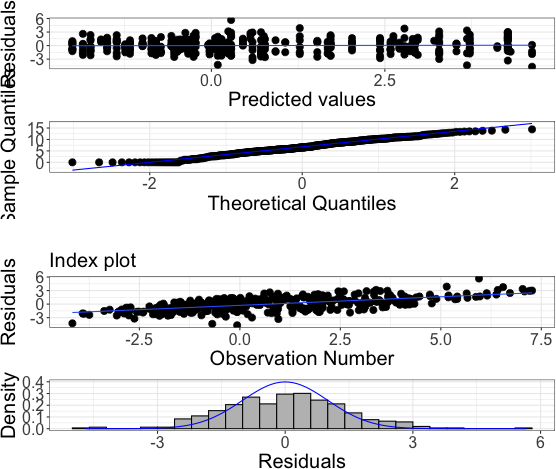
\includegraphics[width=1\linewidth]{AppendixC_model_diagnosis_files/figure-latex/indiv-biom-18-1} \caption{Diagnosis plot for a model of crop identity and corn weed management effects on individual biomass.}\label{fig:indiv-biom-18}
\end{figure}

\begin{Shaded}
\begin{Highlighting}[]
\DocumentationTok{\#\#\#\# Did crop identity and corn weed management affect individual fecundity? \{{-}\} }

\CommentTok{\# Keep rows with no NAs only, fecundity18\_s for Number of seeds}
\NormalTok{fecundity18\_s }\OtherTok{\textless{}{-}}\NormalTok{ fecundity18[}\FunctionTok{complete.cases}\NormalTok{(fecundity18}\SpecialCharTok{$}\NormalTok{Seed), ]}

\CommentTok{\# min(fecundity18\_s$Seed[fecundity18\_s$Seed \textgreater{} 0])}

\NormalTok{seeds.gls }\OtherTok{\textless{}{-}} \FunctionTok{gls}\NormalTok{(}\FunctionTok{log}\NormalTok{(Seed }\SpecialCharTok{+} \DecValTok{1}\NormalTok{) }\SpecialCharTok{\textasciitilde{}}\NormalTok{ Block }\SpecialCharTok{+} 
\NormalTok{                   Crop\_ID}\SpecialCharTok{*}\NormalTok{Corn\_weed\_management,}
                 \AttributeTok{correlation=}\FunctionTok{corCompSymm}\NormalTok{(}\AttributeTok{form=} \SpecialCharTok{\textasciitilde{}}\DecValTok{1} \SpecialCharTok{|}\NormalTok{ bt), }\CommentTok{\#identifies each treatment within block}
  \AttributeTok{data=}\NormalTok{fecundity18\_s)}

\FunctionTok{diag\_seed}\NormalTok{(seeds.gls , }\AttributeTok{tag=} \StringTok{""}\NormalTok{)}
\end{Highlighting}
\end{Shaded}

\begin{figure}
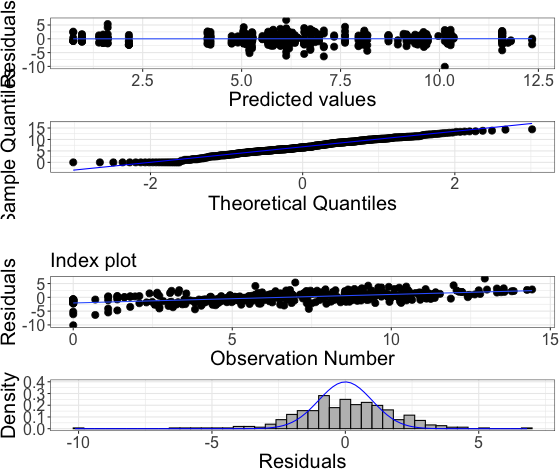
\includegraphics[width=1\linewidth]{AppendixC_model_diagnosis_files/figure-latex/indiv-seed-18-1} \caption{Diagnosis plot for a model of crop identity and corn weed management effect on individual fecundity.}\label{fig:indiv-seed-18}
\end{figure}

\begin{Shaded}
\begin{Highlighting}[]
\DocumentationTok{\#\#\# 18{-}mean full compound symmetry model}
\DocumentationTok{\#\#\#\# Did crop identity, corn weed management, and individual aboveground mass affect AMATA aboveground mass in 2018? \#\#\#\# }
\NormalTok{fecundity18\_sb }\OtherTok{\textless{}{-}}\NormalTok{ fecundity18[}\FunctionTok{complete.cases}\NormalTok{(fecundity18}\SpecialCharTok{$}\NormalTok{Seed, fecundity18}\SpecialCharTok{$}\NormalTok{Biomass), ]}

\CommentTok{\#log(fecundity18\_sb$Biomass )}
\NormalTok{allcrops.biom.seed.gls }\OtherTok{\textless{}{-}} \FunctionTok{gls}\NormalTok{(}\FunctionTok{log}\NormalTok{(Seed}\SpecialCharTok{+}\DecValTok{1}\NormalTok{) }\SpecialCharTok{\textasciitilde{}}\NormalTok{ Block }\SpecialCharTok{+} \FunctionTok{log}\NormalTok{(Biomass }\SpecialCharTok{+} \FloatTok{0.005}\NormalTok{) }\SpecialCharTok{+} 
\NormalTok{                                Crop\_ID }\SpecialCharTok{+}\NormalTok{ Corn\_weed\_management }\SpecialCharTok{+}
\NormalTok{                      Crop\_ID}\SpecialCharTok{:}\NormalTok{Corn\_weed\_management }\SpecialCharTok{+}
\NormalTok{                      Crop\_ID}\SpecialCharTok{:}\FunctionTok{log}\NormalTok{(Biomass }\SpecialCharTok{+} \FloatTok{0.005}\NormalTok{) }\SpecialCharTok{+} 
\NormalTok{                        Corn\_weed\_management}\SpecialCharTok{:}\FunctionTok{log}\NormalTok{(Biomass }\SpecialCharTok{+} \FloatTok{0.005}\NormalTok{) }\SpecialCharTok{+}
\NormalTok{                      Crop\_ID}\SpecialCharTok{:}\NormalTok{Corn\_weed\_management}\SpecialCharTok{:}\FunctionTok{log}\NormalTok{(Biomass }\SpecialCharTok{+} \FloatTok{0.005}\NormalTok{),}
  \AttributeTok{correlation=}\FunctionTok{corCompSymm}\NormalTok{(}\AttributeTok{form=} \SpecialCharTok{\textasciitilde{}}\DecValTok{1} \SpecialCharTok{|}\NormalTok{ bt), }\CommentTok{\#identifies each treatment within block}
  \AttributeTok{data=}\NormalTok{fecundity18\_sb)}

\FunctionTok{diag\_seed}\NormalTok{(allcrops.biom.seed.gls, }\AttributeTok{tag =} \StringTok{""}\NormalTok{) }
\end{Highlighting}
\end{Shaded}

\begin{figure}
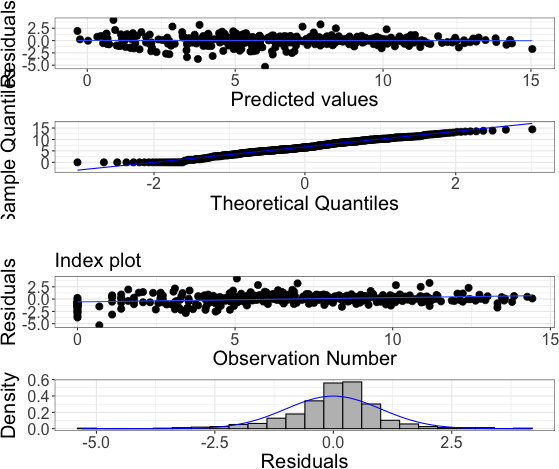
\includegraphics[width=1\linewidth]{AppendixC_model_diagnosis_files/figure-latex/indiv-biom-seed-18-1} \caption{Diagnosis plot for a model of crop identity and corn weed management effect on individual fecundity.}\label{fig:indiv-biom-seed-18}
\end{figure}

\end{document}
